\chapter{Cooling}
\label{chapter:cooling-only}

In this chapter, we document a test case configured with a zero wind
stress and constant negative heat flux
\begin{equation}
Q=-100~\mbox{W}~\mbox{m}^{-2}.
\end{equation}
Temperature is initialized with a stable linear stratification
according to equation (\ref{eq:linear-stratification}).  Cooling acts
to deepen the boundary layer and thus to eat away at the linear
stratification. Given the zero wind stress forcing, and zero lateral
gradients, the velocity remains unchanged from its initial zero value.
This test exercises the local downgradient diffusive portion of KPP as
well as the non-local KPP transport.


\section{Results from GFDL-MOM6}
\label{section:winds_and_cooling_mom6}

Figure \ref{fig:MOM6_SST_bldepth-cooling} shows the KPP boundary layer
depth, mixed layer depth, and SST from the MOM6 implementation of
CVMix/KPP.  The boundary layer and mixed layer deepen steadily
throughout the simulation, with the SST cooling.  This behaviour is
reflected in Figure \ref{fig:MOM6_temp-cooling}, which shows the depth
profile of temperature.  Note how the four simulations track one
another rather closely, much more closely than the tests with
wind-alone (Chapter \ref{chapter:wind_alone}) or winds plus positive
surface heat flux (Chapter \ref{chapter:winds_and_heating}).

The KPP diffusivity is shown in Figure
\ref{fig:MOM6_KPP_diffusivity-cooling}, with each grid showing the
same characteristics of a steadily increasing value, with the increase
associated with the deepening boundary layer depth. Again, the four
simulations exhibit similar characteristics.  The KPP non-local
transport is shown in Figure \ref{fig:MOM6_KPP_nonlocal-cooling}.
Each grid shows the same characteristics, with a warming near the
surface and cooling towards the lower portion of the boundary layer.
This behaviour is consistent with the default profile of the non-local
contribution to KPP in the CVMix scheme.  The surface warming arises
from the redistribution of the cooling surface boundary flux
throughout the boundary layer.  That is, the non-local term warms the
top portion of the boundary layer relative to the case without the
non-local term, and cools the lower portion of the boundary layer.
  

%%%%%%%%%%%%%%%%%%%% %%%%%%%%%%%%%%%%%%%%%%%%%
\begin{figure}[h!t]
%\rule{\textwidth}{0.005in}
\begin{center}
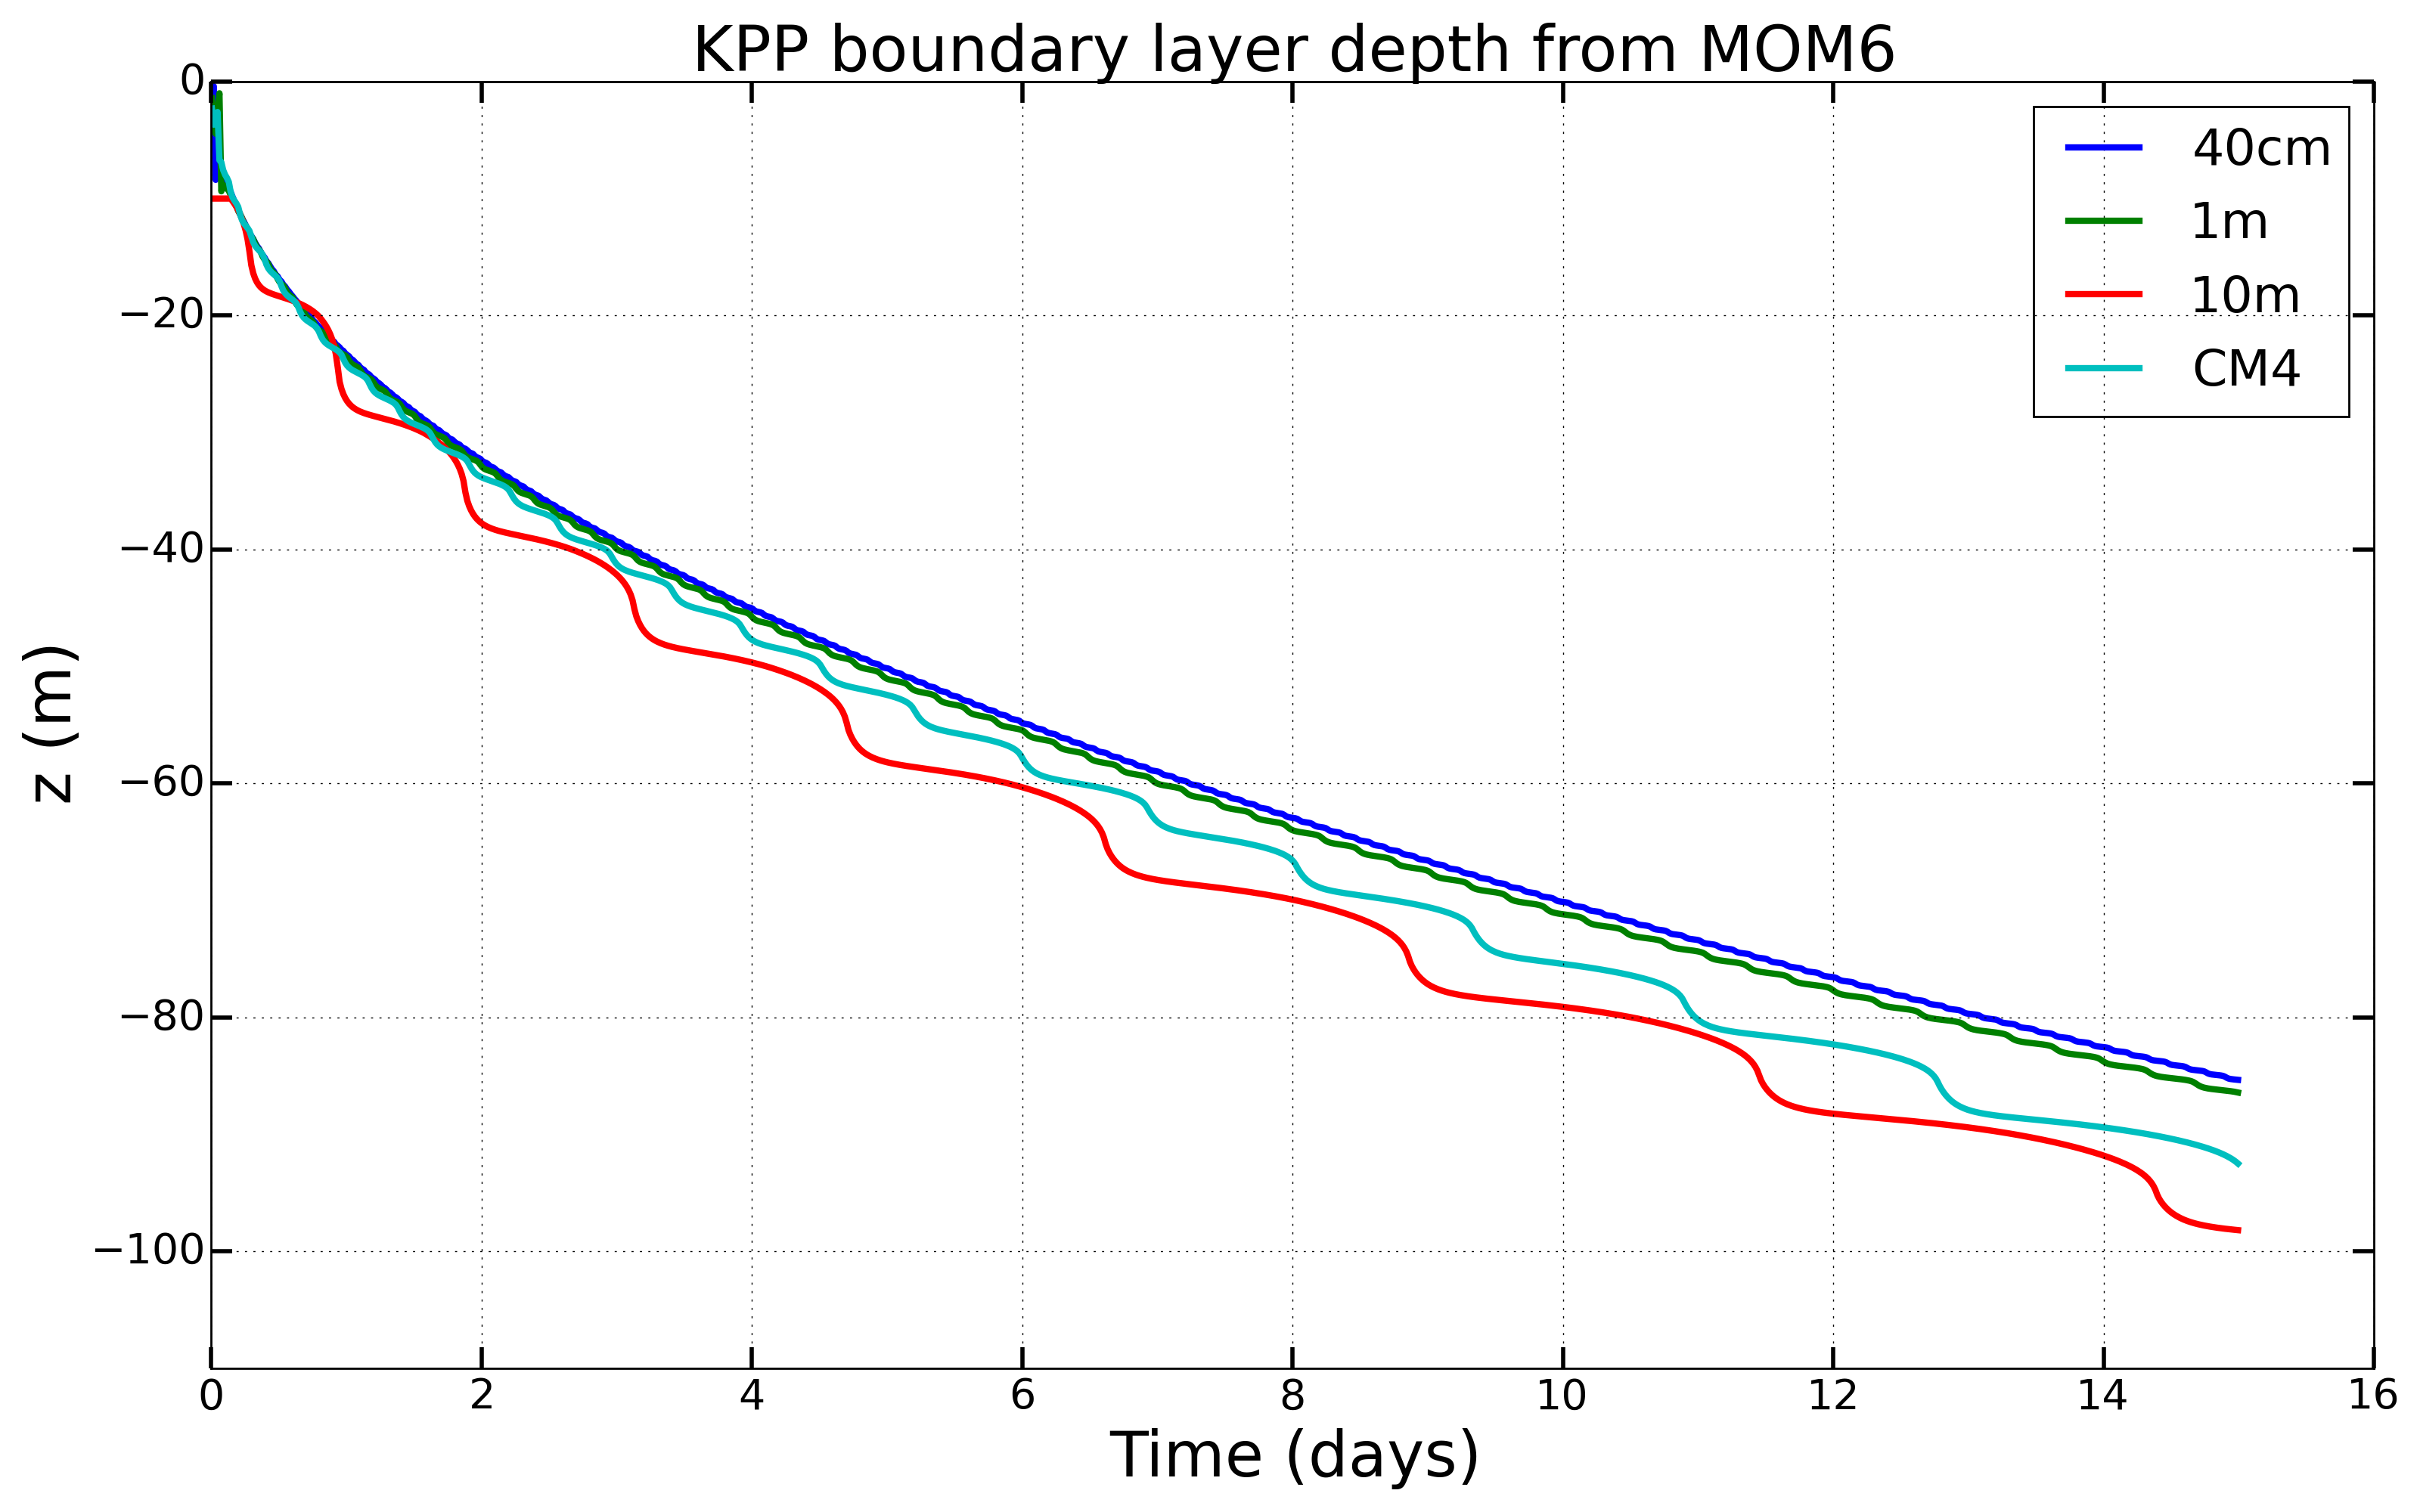
\includegraphics[angle=0,width=5cm]{./figs/MOM6/cooling_KPP_MOM6_bldepth.png}
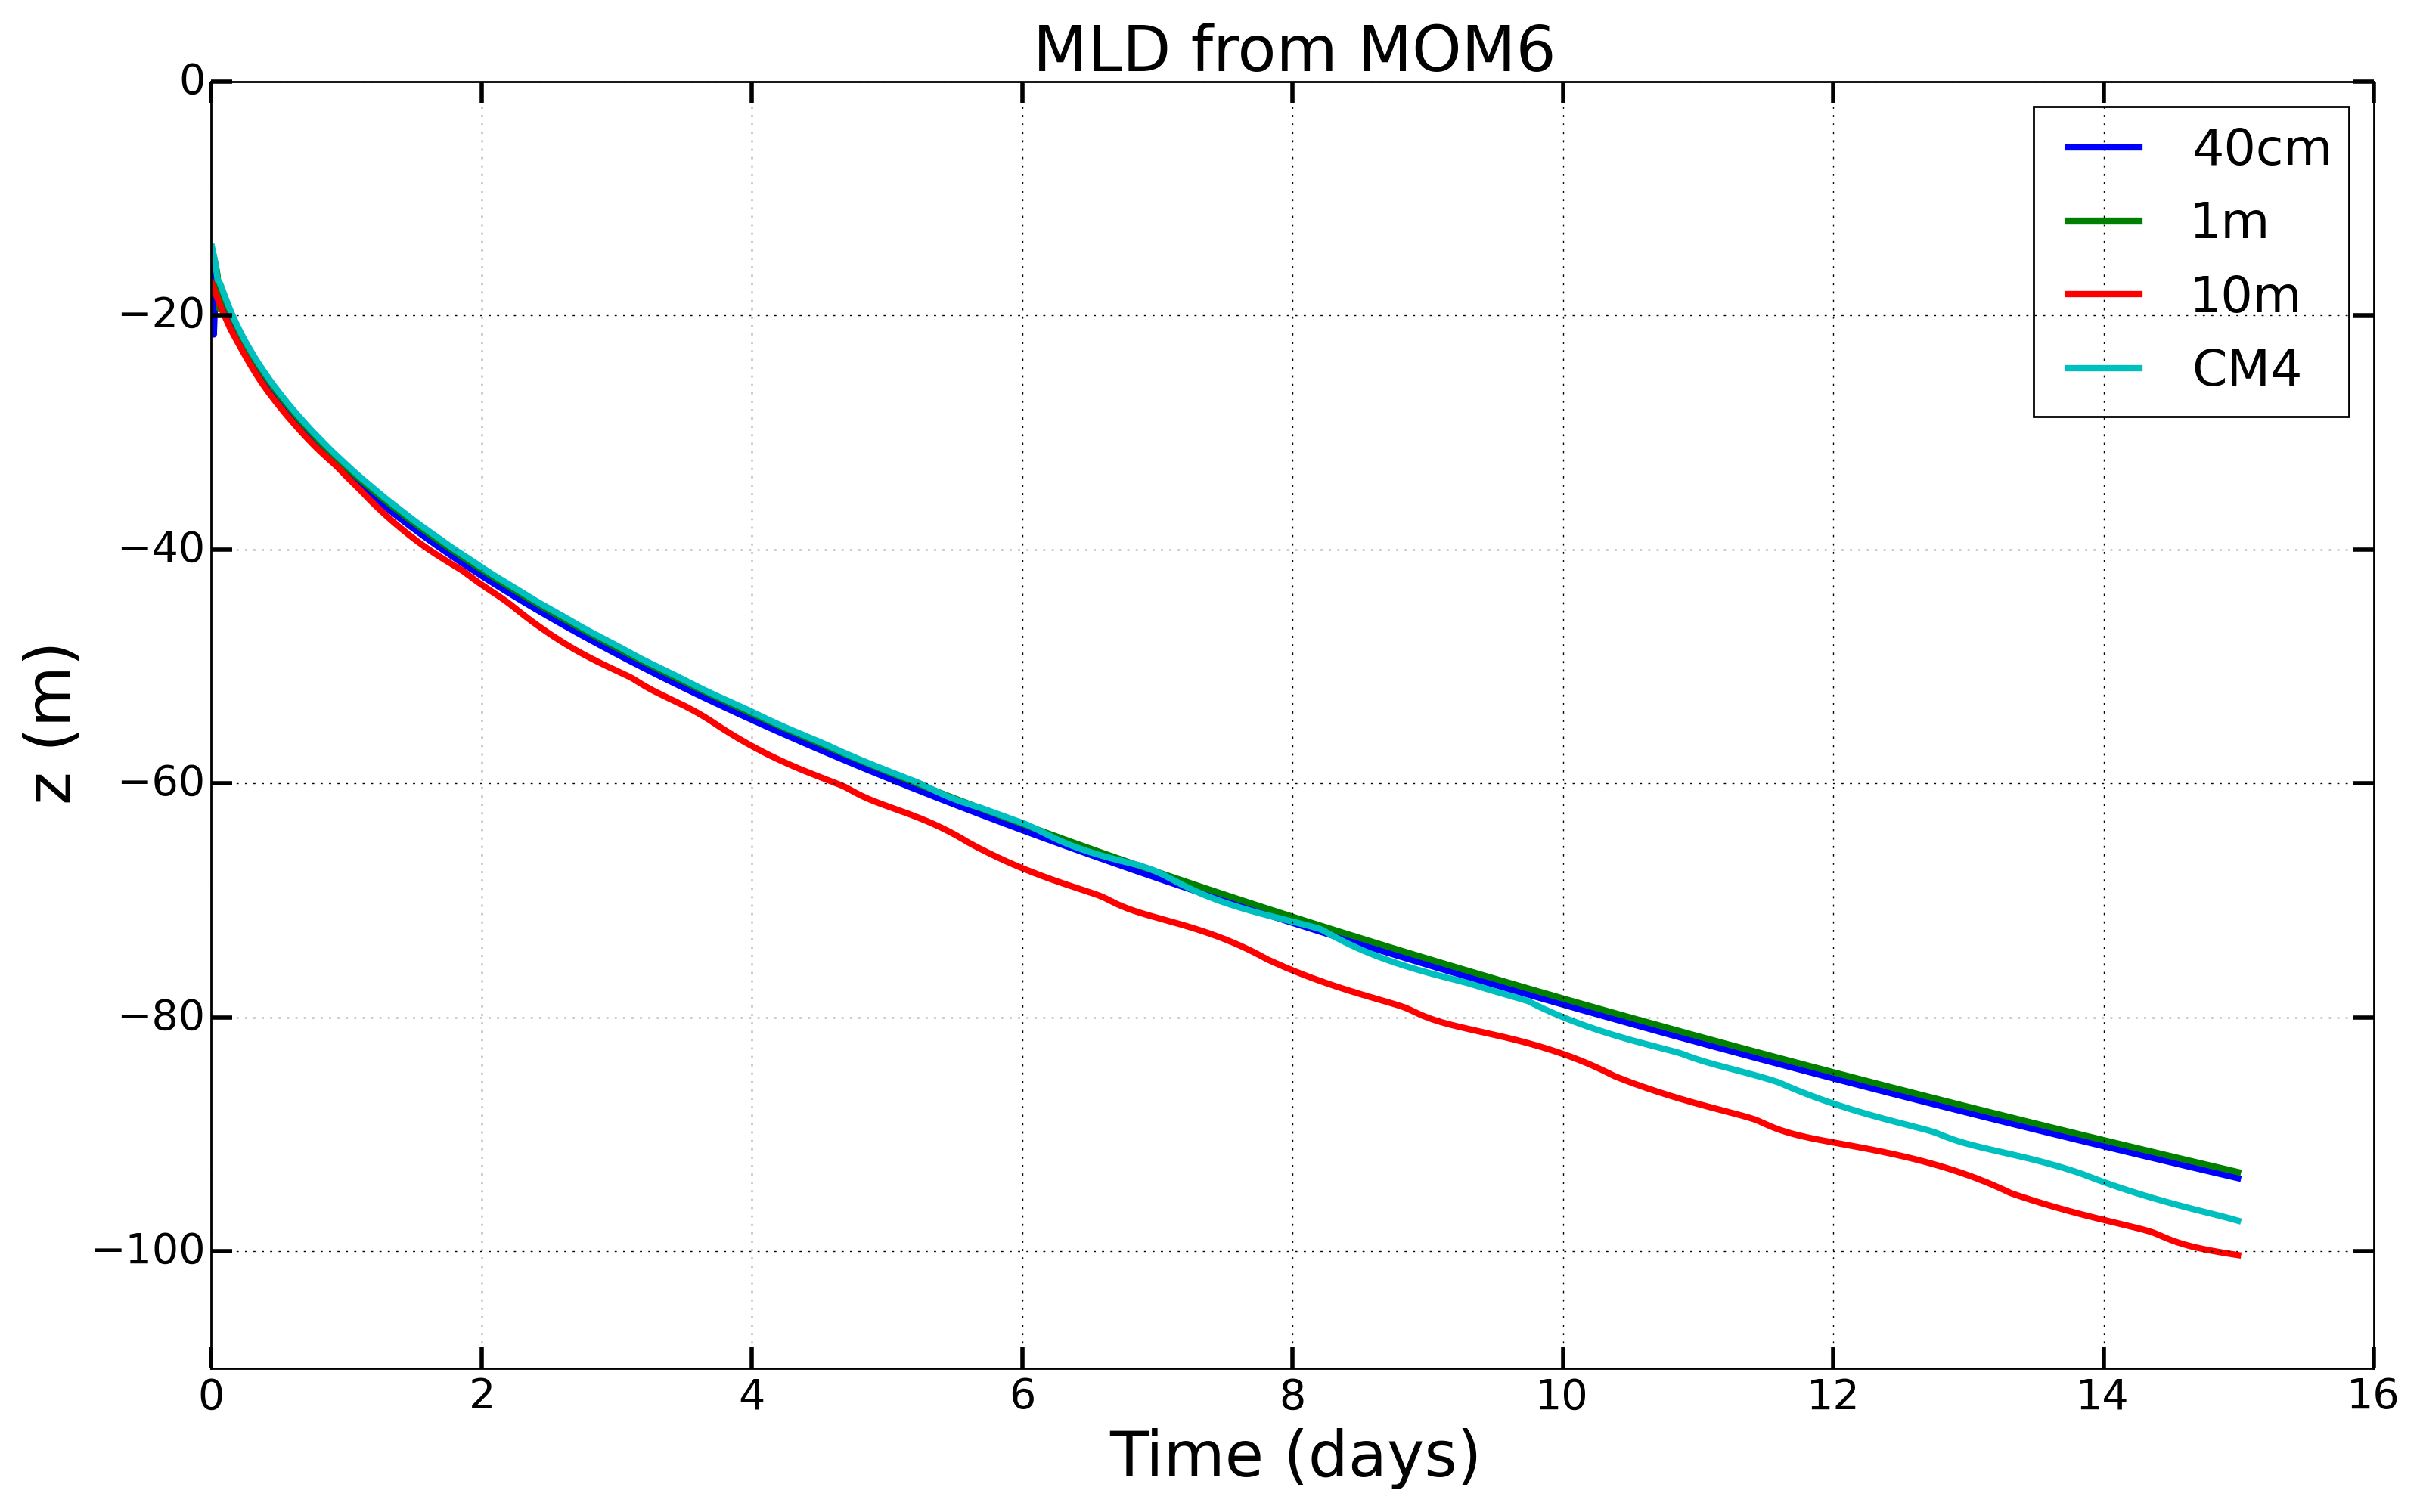
\includegraphics[angle=0,width=5cm]{./figs/MOM6/cooling_KPP_MOM6_mld.png}
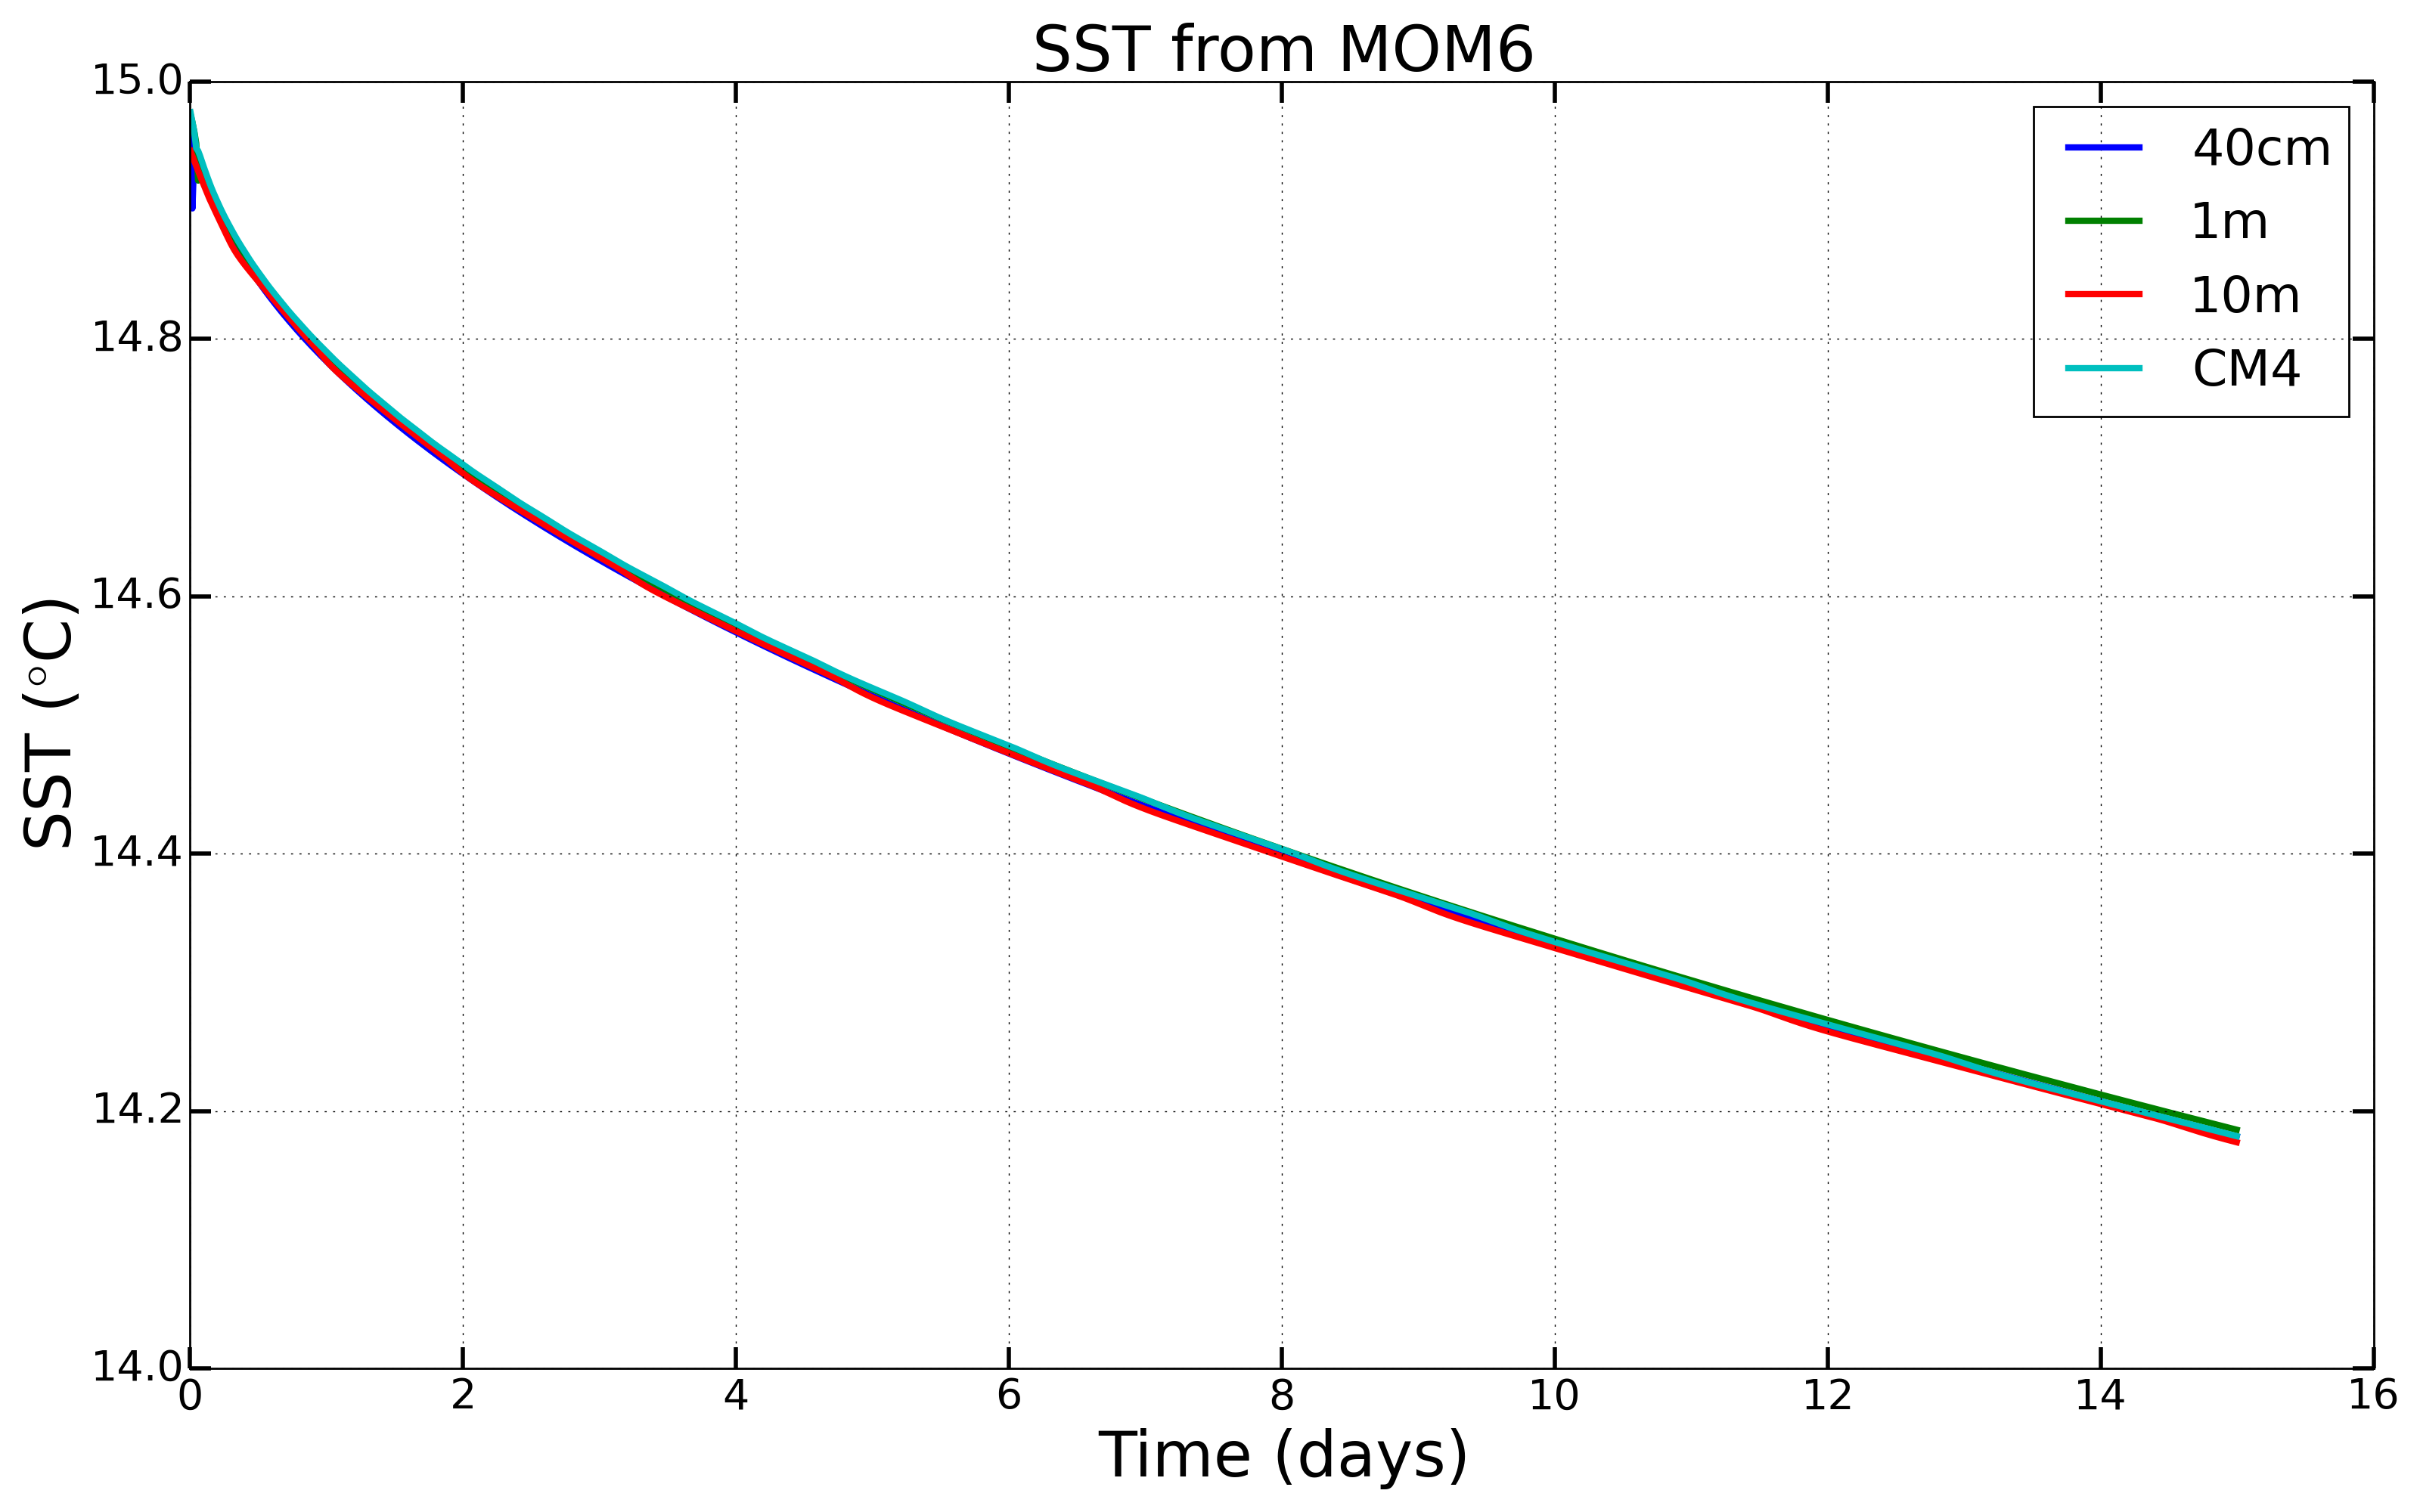
\includegraphics[angle=0,width=5cm]{./figs/MOM6/cooling_KPP_MOM6_SST.png}
\caption[KPP BL depth, ML depth, and SST from MOM6 for cooling
test]{\sf Time series for KPP boundary layer depth (left panel), mixed
  layer depth (middle panel), and SST (right panel) for the cooling
  test case (zero winds and $Q=-100~\mbox{W}~\mbox{m}^{-2}$) as
  realized in MOM6.  The mixed layer depth is diagnosed as the depth
  where density differs from the surface by
  $0.003~\mbox{kg}~\mbox{m}^{-3}.$}
\label{fig:MOM6_SST_bldepth-cooling}
\end{center}
%\rule{\textwidth}{0.005in}
\end{figure}
%%%%%%%%%%%%%%%%%%%%%%%%%%%%%%%%%%%%%%%%%%%%%%%%%%%%%%%%%%%%%%%%%%%%%%%%

%%%%%%%%%%%%%%%%%%%% %%%%%%%%%%%%%%%%%%%%%%%%%
\begin{figure}[h!t]
%\rule{\textwidth}{0.005in}
\begin{center}
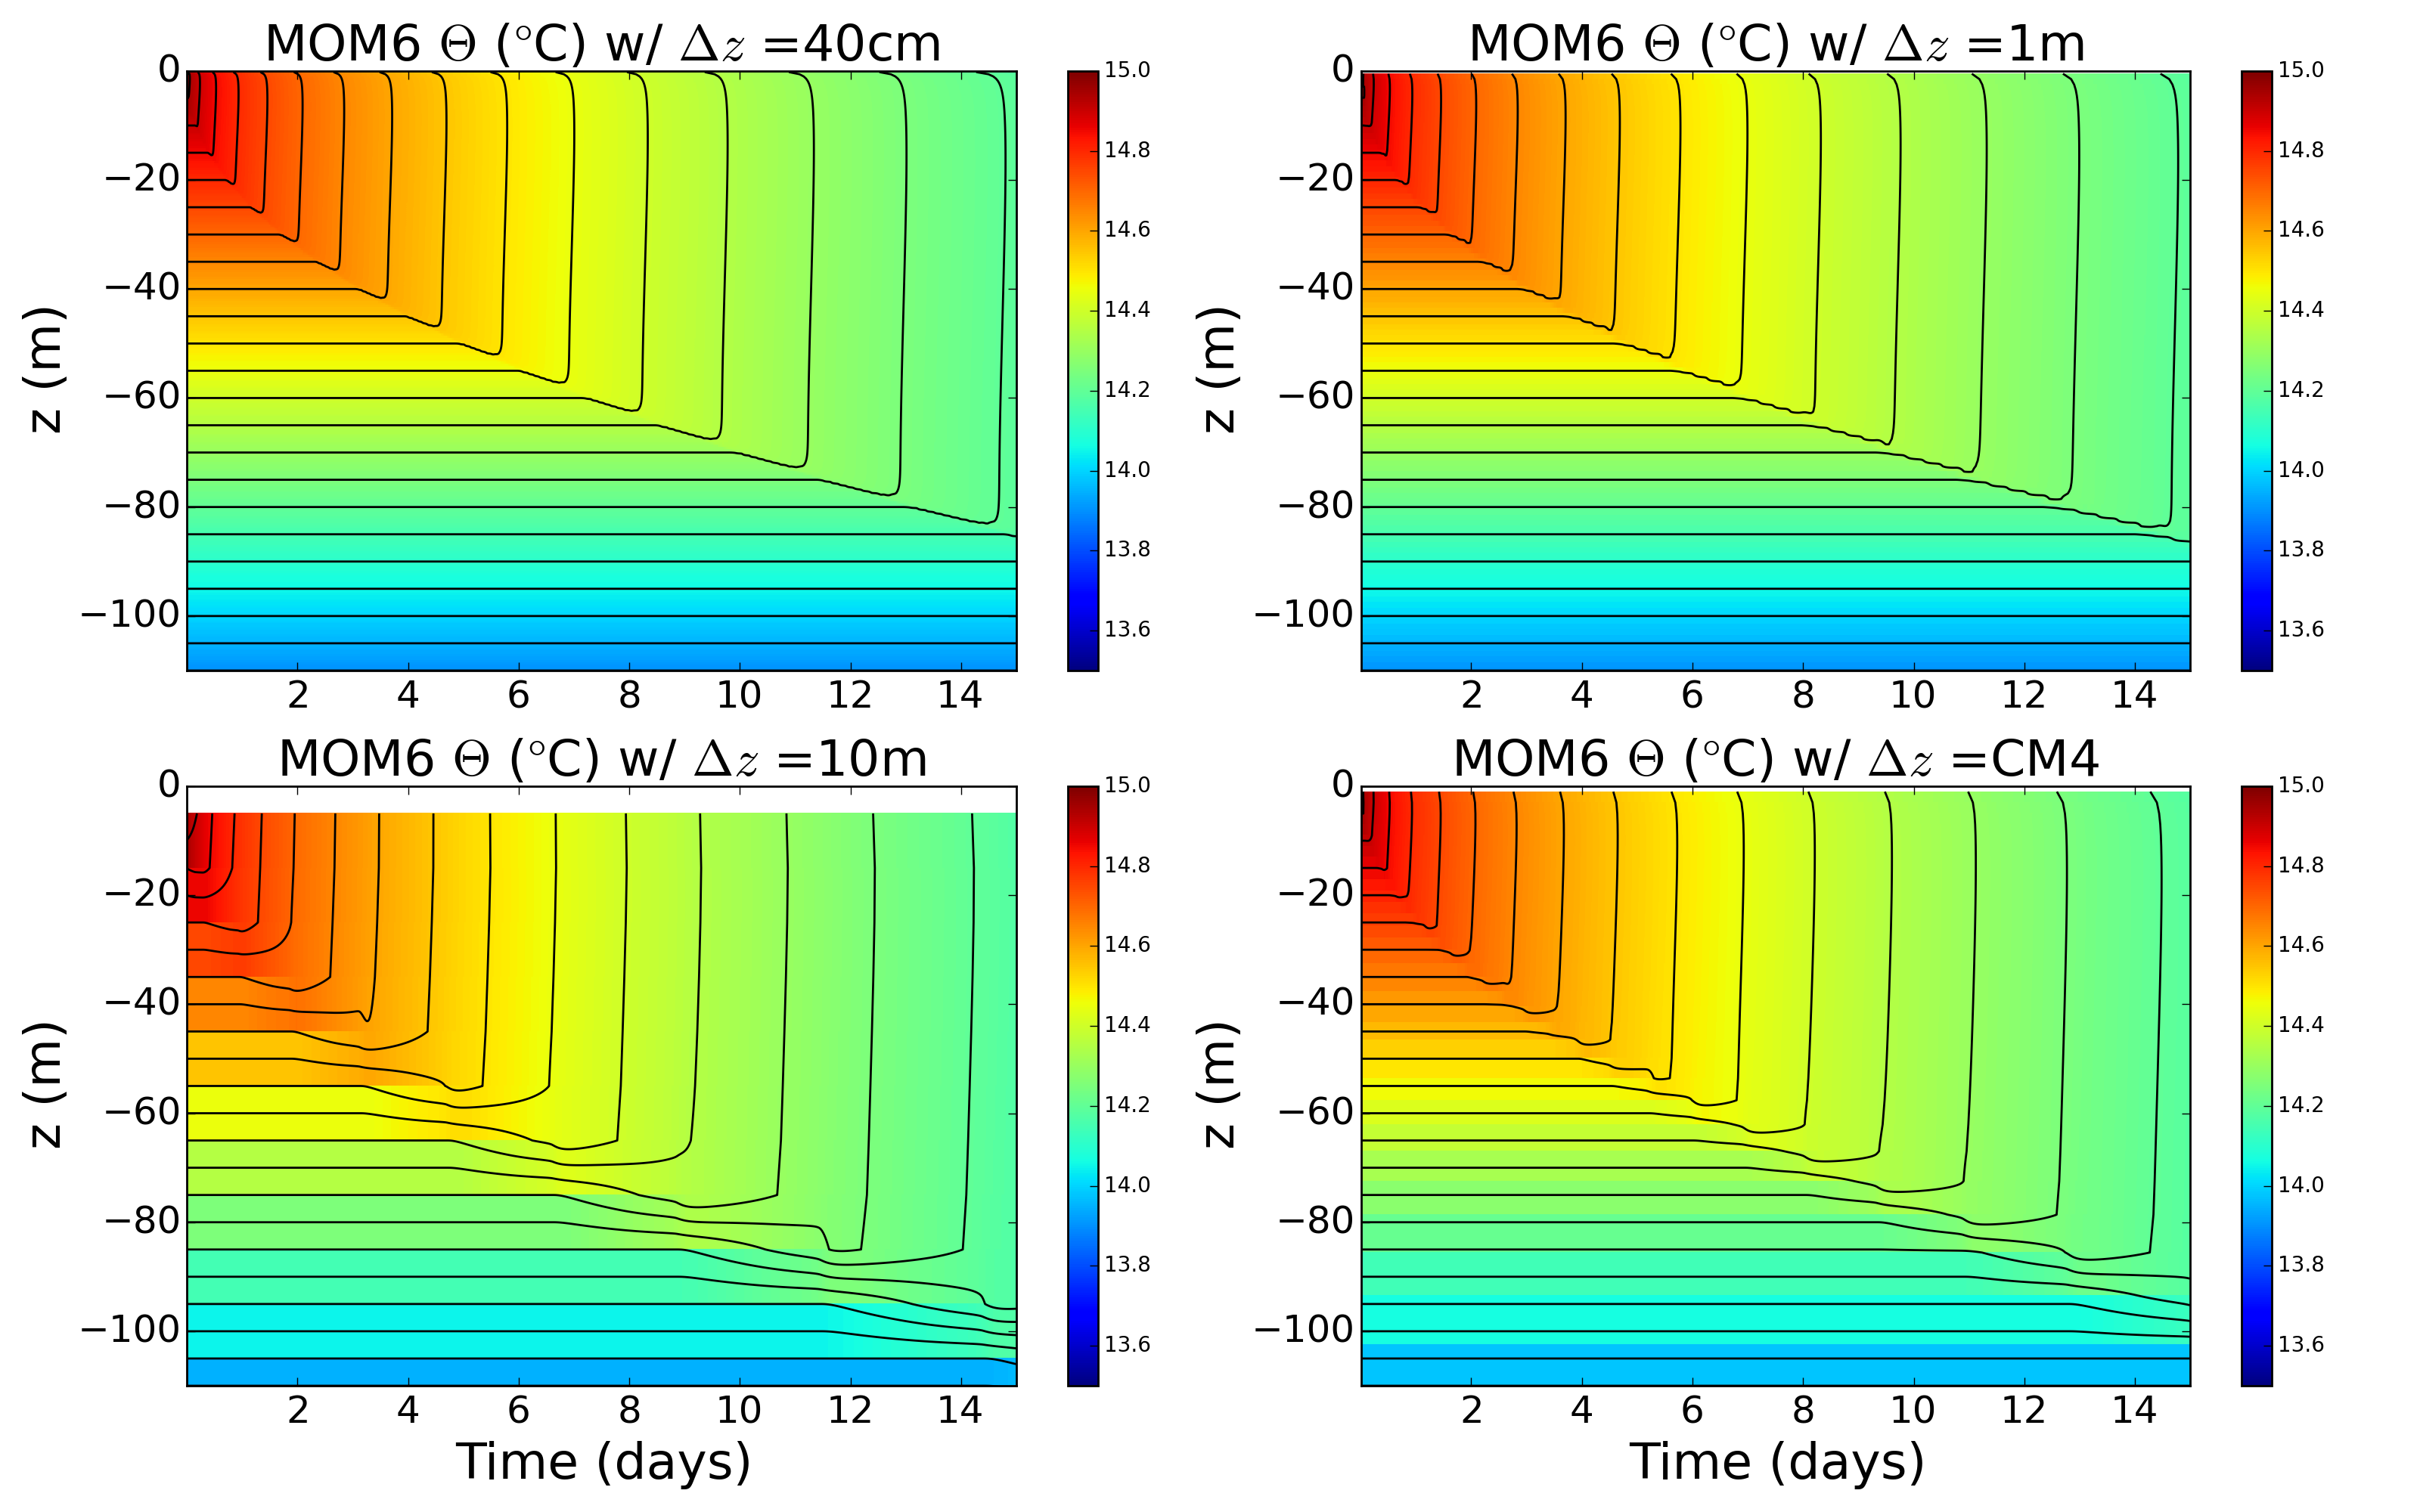
\includegraphics[angle=0,width=14cm]{./figs/MOM6/cooling_KPP_MOM6_temp.png}
\caption[Temperature from MOM6 for cooling test]{\sf Time series for
  temperature from cooling test case (zero wind stress and
  $Q=-100~\mbox{W}~\mbox{m}^{-2}$) as realized in MOM6 using four
  different vertical grid resolutions.}
\label{fig:MOM6_temp-cooling}
\end{center}
%\rule{\textwidth}{0.005in}
\end{figure}
%%%%%%%%%%%%%%%%%%%%%%%%%%%%%%%%%%%%%%%%%%%%%%%%%%%%%%%%%%%%%%%%%%%%%%%%


%%%%%%%%%%%%%%%%%%%% %%%%%%%%%%%%%%%%%%%%%%%%%
\begin{figure}[h!t]
%\rule{\textwidth}{0.005in}
\begin{center}
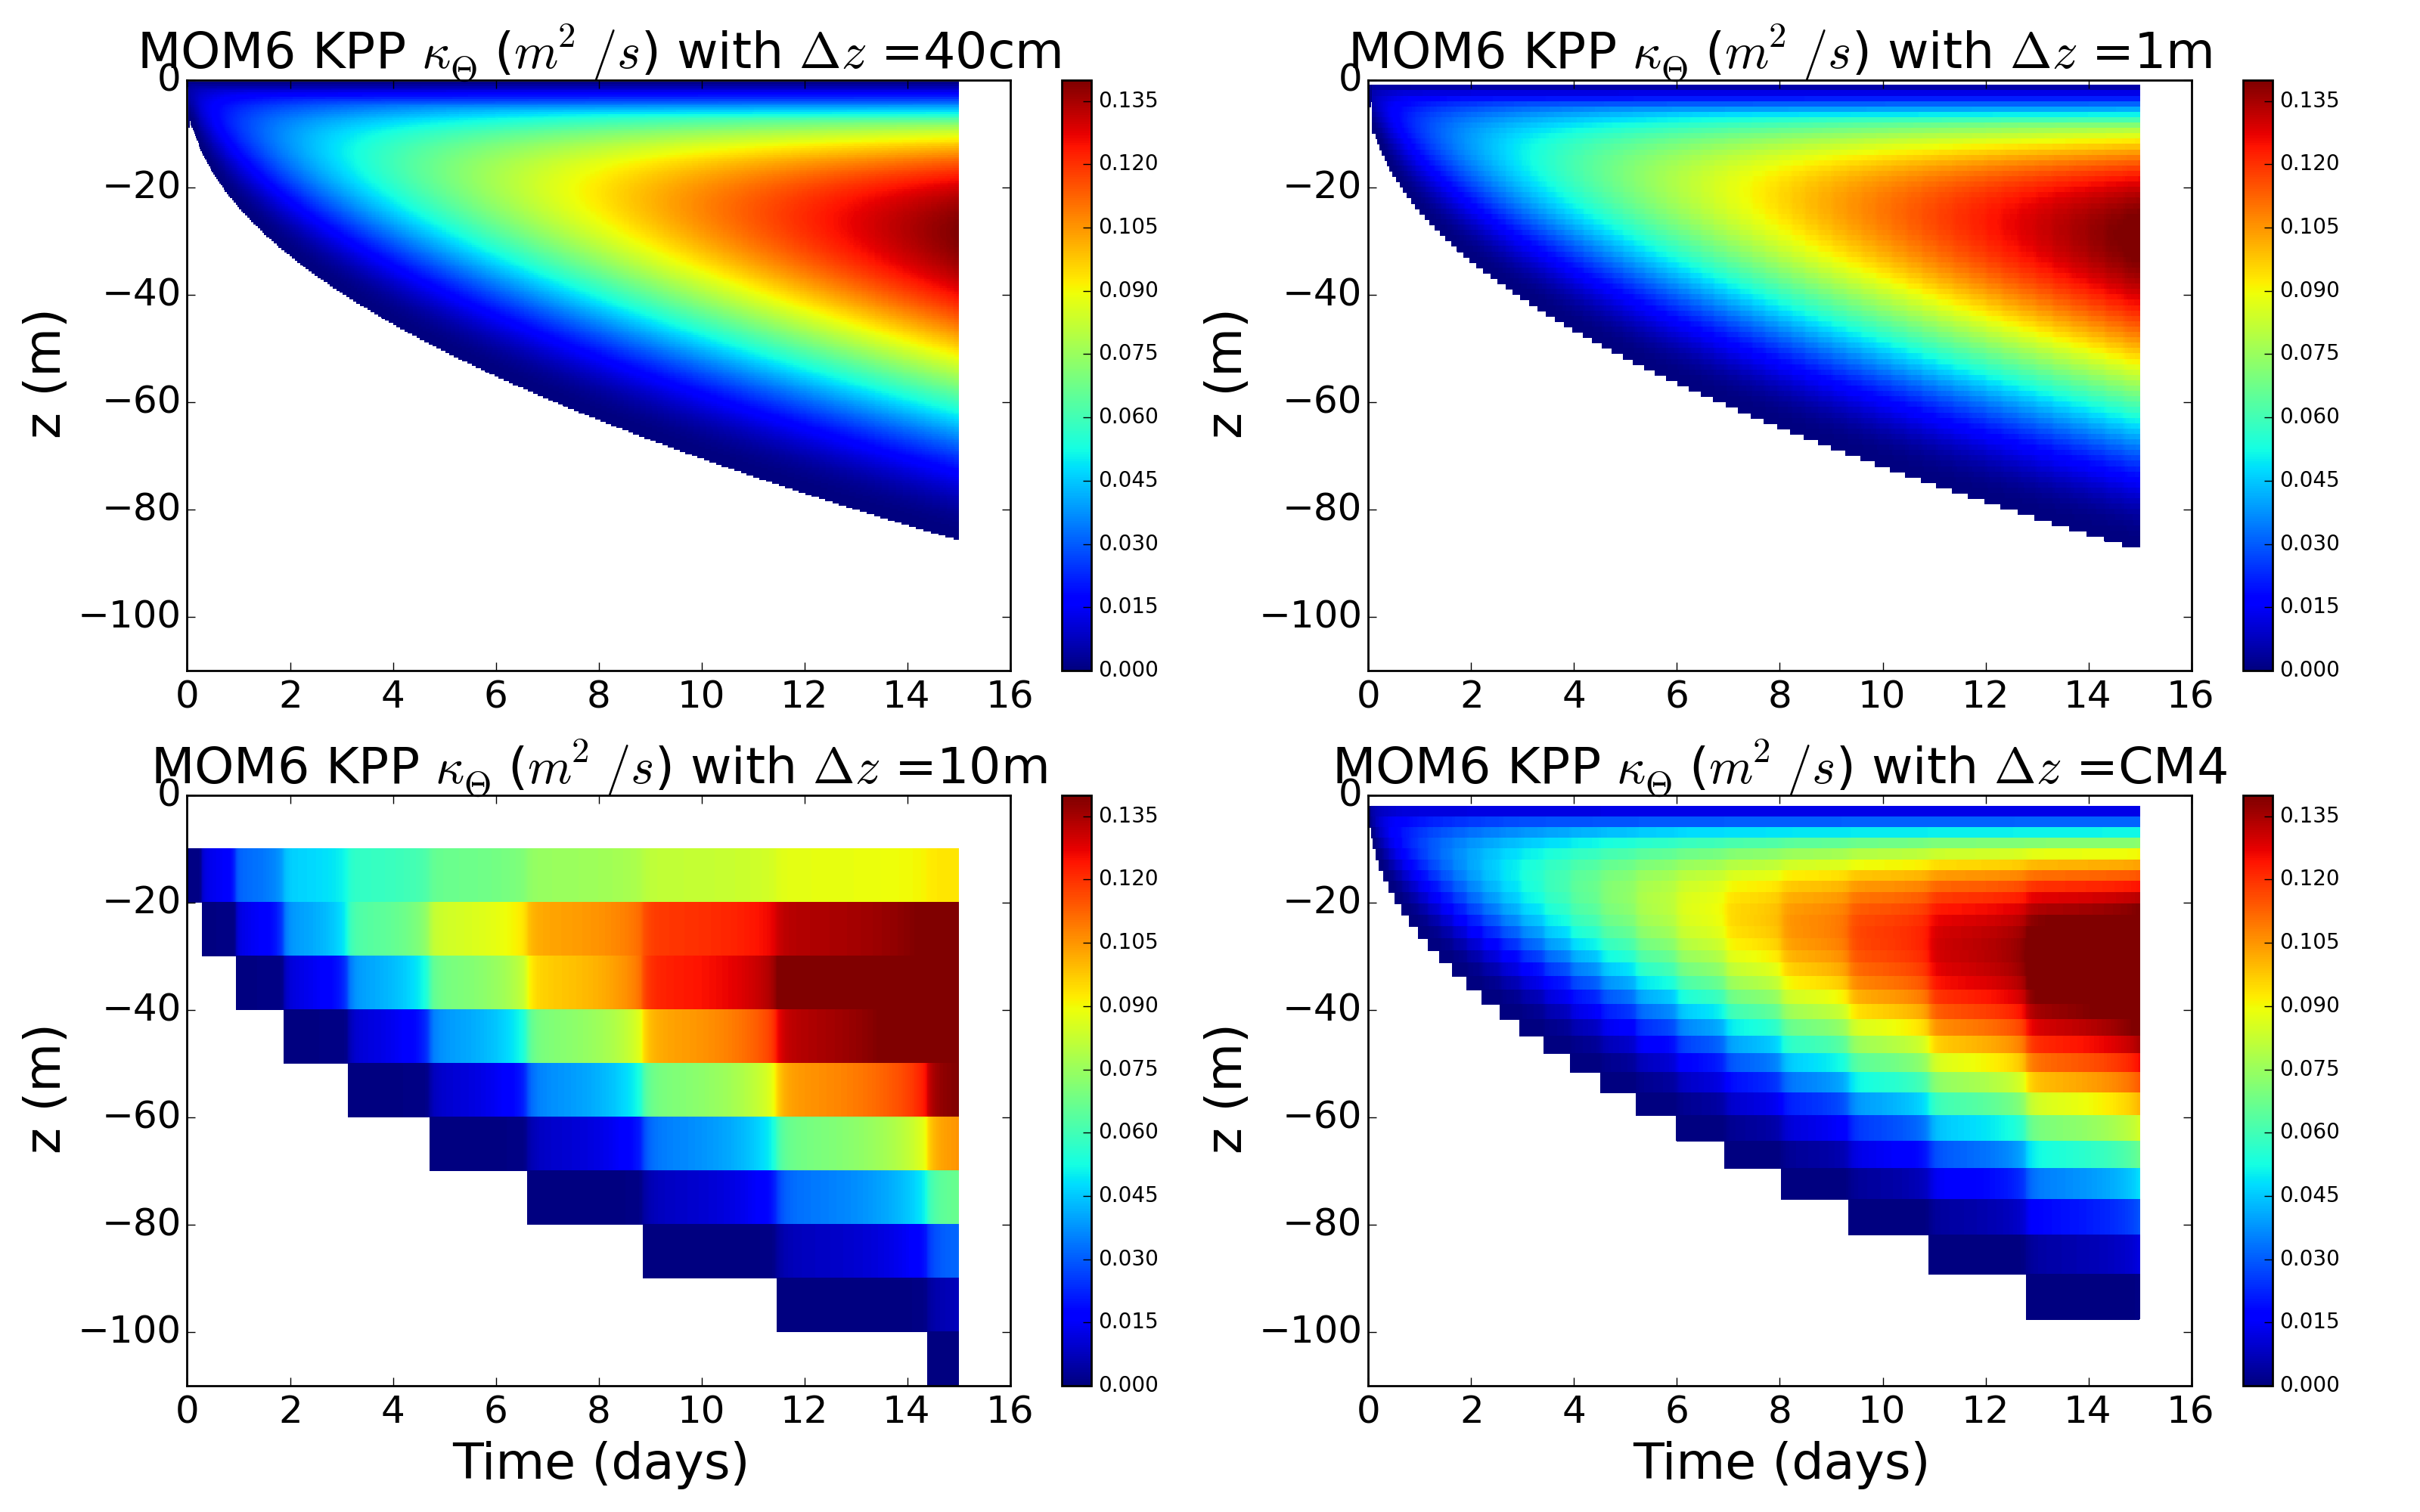
\includegraphics[angle=0,width=14cm]{./figs/MOM6/cooling_KPP_MOM6_KPP_diffusivity.png}
\caption[KPP diffusivity from MOM6 for cooling test]{\sf Time series
  for the KPP vertical diffusivity for cooling test case (zero wind
  stress and $Q=100~\mbox{W}~\mbox{m}^{-2}$) as realized in MOM6 using
  four different vertical grid resolutions.}
\label{fig:MOM6_KPP_diffusivity-cooling}
\end{center}
%\rule{\textwidth}{0.005in}
\end{figure}
%%%%%%%%%%%%%%%%%%%%%%%%%%%%%%%%%%%%%%%%%%%%%%%%%%%%%%%%%%%%%%%%%%%%%%%%


%%%%%%%%%%%%%%%%%%%% %%%%%%%%%%%%%%%%%%%%%%%%%
\begin{figure}[h!t]
%\rule{\textwidth}{0.005in}
\begin{center}
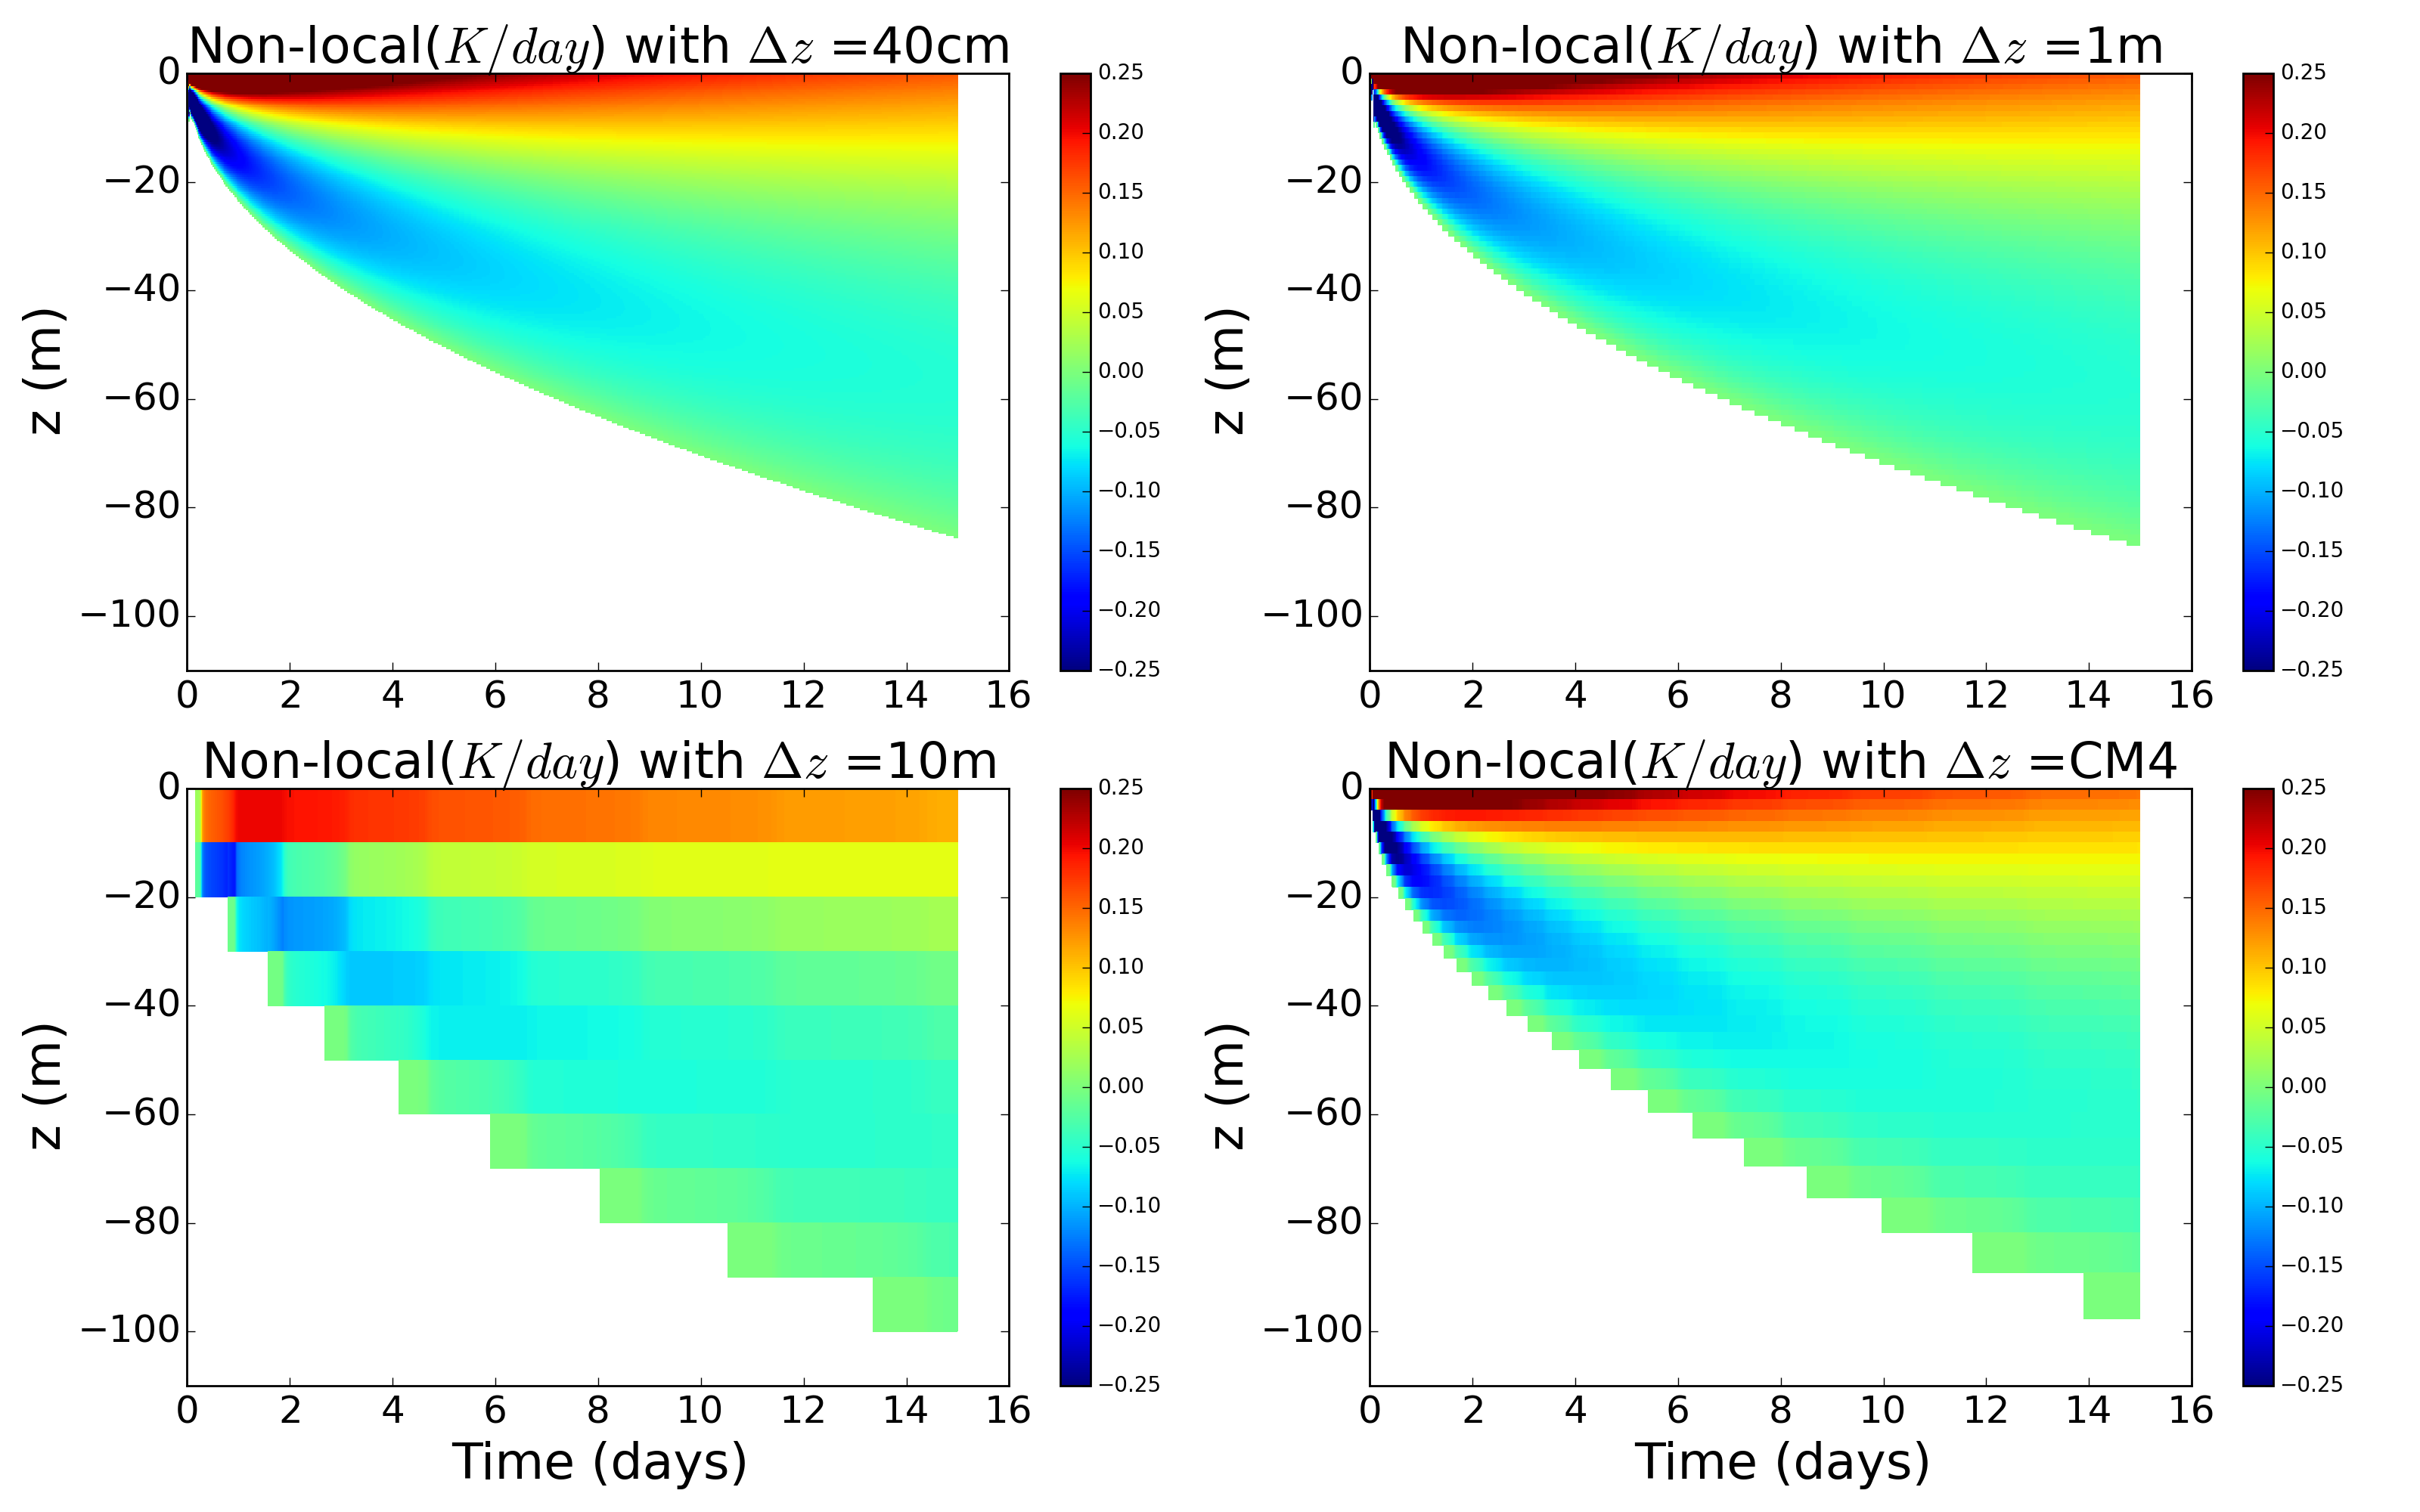
\includegraphics[angle=0,width=14cm]{./figs/MOM6/cooling_KPP_MOM6_nonlocal_temp_tendency.png}
\caption[KPP nonlocal time tendency from MOM6 cooling test]{\sf Time
  series for the time tendency from the KPP non-local transport for
  the cooling test case (zero wind stress and
  $Q=100~\mbox{W}~\mbox{m}^{-2}$) as realized in MOM6 using four
  different vertical grid resolutions.}
\label{fig:MOM6_KPP_nonlocal-cooling}
\end{center}
%\rule{\textwidth}{0.005in}
\end{figure}
%%%%%%%%%%%%%%%%%%%%%%%%%%%%%%%%%%%%%%%%%%%%%%%%%%%%%%%%%%%%%%%%%%%%%%%%



